\section{Data description}\label{sec:data}
\subsection{Sources and universe}
All data are public. The universe is the members of the S\&P~100 and the EURO STOXX~50 on 31 December 2014, the day before the test period, so membership is not chosen with hindsight. Of these 150 firms (100 and 50), nine lack a usable price history in the free data and are excluded: eight were acquired, merged or taken private between 2016 and 2025, and one has only a stale secondary listing. This leaves \Firms{} firms, \FirmsUS{} in the United States and \FirmsEU{} in the euro area, in ten sectors (Appendix~\ref{app:universe}). The exclusion uses later information; it affects 6\% of the names, and the sign of the bias is unknown because takeover targets often gain when a bid is announced. Unilever is represented by its London line, as its Amsterdam line ended with the 2020 unification.

Daily prices, volume, exchange rates and the MSCI World benchmark (the URTH fund, with dividends) come from Yahoo Finance from 2005, and the risk-free rate is the three-month U.S. Treasury yield. Returns are in U.S. dollars, unhedged. Vivendi leaves the universe at its December 2024 break-up.

Headlines come from Google News searches on each company's name, one query per firm and calendar month from October 2010 to December 2025, retrieved in October 2026. Google returns at most 100 items per query, so heavily covered firms are sampled.

\subsection{Preparation and quality}
Figure~\ref{fig:retention} shows how \Retrieved{} retrieved items become \Headlines{} company headlines. Duplicates are removed, and a headline is kept only if it names the issuer. Names that are also common words or people, such as Apple or Ford, must appear together with business words. Market roundups naming three or more firms (\Roundups{} headlines) are removed.
\end{multicols}
\begin{figure}[H]\centering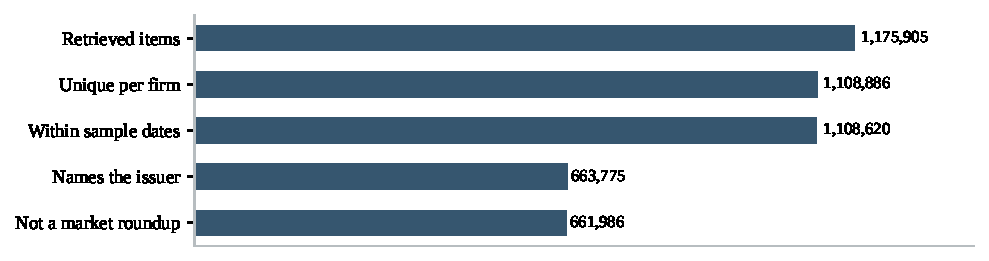
\includegraphics[width=\textwidth]{retention}
\caption{Headline retention from retrieval to the weekly decision panel.}\label{fig:retention}\end{figure}
\begin{multicols}{2}

Most headlines are close to neutral, while about \TonePositiveShare{} are clearly positive and \ToneNegativeShare{} clearly negative ($|s|>0.5$; Figure~\ref{fig:tone}). Euro-area headlines are more positive than U.S. headlines, and tone rose after 2020; such level differences are why tone is measured against each firm's own history.
\end{multicols}
\begin{figure}[H]\centering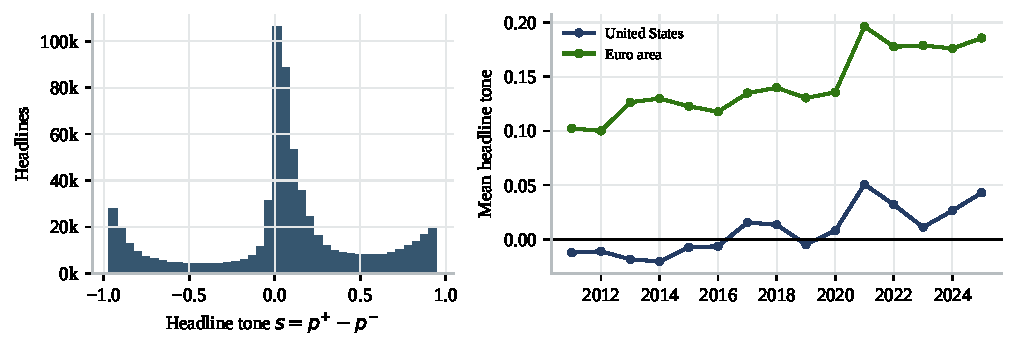
\includegraphics[width=\textwidth]{tone}
\caption{FinBERT tone of the accepted headlines: distribution (left) and annual mean by region (right).}\label{fig:tone}\end{figure}
\begin{multicols}{2}

Google News reports only the publication date, so a headline counts only from the next opening of the issuer's exchange. Coverage is uneven across firms and sectors (Figure~\ref{fig:coverage}); the median firm has \MedianHeadlinesWeek{} headlines a week, and no news arrives in \NoNewsShare{} of test stock-weeks, which then carry neutral sentiment.
